\chapter{Methodology}
\label{chap:methodology}

This chapter describes the proposed data analytics workflow.
Besides, the QoS data gathering procedures are briefly presented,
and the proposed system is compared with previous projects.

\section{Measurement Process}

The time series used in this work represent network end-to-end measures of a
cable-television infrastructure, which runs DOCSIS with asymmetric download and
upload bandwidths. A home router connected to a cable modem communicates
with a server strategically located by the ISP\@. Each server is responsible
for measurements of several end-users.
Measurements are triggered in
each home router every half hour and, by the end of every day,
the results are transferred to a database.
The software responsible for these procedures was
developed by TGR (a startup at UFRJ),
and is spread over approximately X thousand customers of a major Brazilian
Tier-3 ISP\@.

To measure the round
trip packet loss fraction and the RTT between the home router and the associated
server, the
home router sends a train of short UDP packets, and the server bounces back
them. The data here presented considers a train of 100 UDP packets of 32 bytes,
separated by 1 millisecond.
Maximum achievable upstream throughput is measured by overflowing the upload
links with parallel TCP data transfers from the end-user to the
server.
Also, the traceroutes from the end-users
to the respective servers are collected with the same frequency. Traceroutes
from servers to end-users are not gathered.
In~\cite{a_preliminary_performance_measurement_study_of_residential_broadband_services_in_brazil}
is presented a preliminary descriptive investigation of these metrics.

The resulted time series are unevenly spaced due to a range of reasons. First,
measurements are initiated only if the residential link is not under use by the
ISP customer. Also, the client may have no Internet connection to start a
measurement, or even be without electrical energy. Other details about the
measurement software are presented during the text, as they are needed.

\section{Pipeline}

This section describes, in a high level abstraction, the proposed workflow
used to detect network events and localize their cause. When necessary, some
steps are better explored in further sections.
The analysis seeks for events during a specific time period, in a single
measurement server, and considers an
particular metric (round trip loss fraction, RTT, or maximum achievable
upstream throughput),
which are specified as parameters.
A complete analysis can be accomplished through different
executions with distinct parameters.
Figure~\ref{fig:pipeline} illustrates the process.

\begin{figure}[H]
    \centering
    \includegraphics[width=0.9\linewidth]{./figures/methodology/pipeline/pipeline.png}
    \caption{Pipeline.}
\label{fig:pipeline}
\end{figure}%

The workflow starts with the End-Users Filtering step,
which aims to remove clients that can negatively affect the analysis.
As an example, this work eliminates clients
with a small number of measurement samples.

The Change Point Detection phase preprocess the end-users time series and
identify change points.
Also, the change points are classified in three types of events: failure,
improvement, or inconclusive. For the RTT and round trip loss fraction,
a change point defines a
failure event if the average of the window after this point is greater than the
average of the window before. The improvement event is analogous, however is
characterized by a mean decrease.
The inconclusive event means that the segments averages are too close.
The same reasoning is applied to maximum
achievable upstream throughput, however, a decrease means a failure, and a
increase is related to an improvement.

The Spatial Correlation procedure clusterizes the end-users in user-groups
according with their position in the network. This clustering can then be used
in further steps to isolate possible events locations.
This stage must produce a specific grouping structure, which is detailed in
Section~\ref{sec:spatial_correlation}.

The Events Times Correlation aims to combine similar events of different
end-users. For example, if three end-users detect a failure at
the same time, then this information is identified at this step.
The grouped end-users events of an user-group are named as network events.
The details of this method are enlightened in
Section~\ref{sec:events_times_correlation}.

Finally, to localize the events cause, the Spatial-Time Correlation method
matches network events with the user-groups structure.
This is better explained in Section~\ref{sec:spatial_time_correlation}.

\section{Spatial Correlation}
\label{sec:spatial_correlation}

This method provides the necessary information to check which network equipment
are shared by end-users that perceive the same network event.
The developed strategies were guided by the specific ISP's topology.

The server position relative to the end-user
can be categorized in two contexts.
In the OFF-NET case, the traffic between them
goes through a Tier-2 ISP\@.
In the ON-NET case, the traffic
doesn't leave the Tier-3 ISP infrastructure.
The latter situation represents a simpler IP topology, since the Tier-3 ISP
uses static routing and
doesn't applies load balancing nor MPLS, techniques that are usual in the Tier-2
ISP network.

Then, considering measurements against a single server and the ON-NET
case, paths from end-users to the server form a hierarchically
structured topology, which is a required design to be consumed by the
Spatial Time Correlation procedure~\ref{sec:spatial_time_correlation}.
This work doesn't have access to the ISP network
topology, therefore, this structure is reconstructed through traceroutes.
In this context, each equipment that responds to traceroute
pings is used as an user-group.
An user-group is formed by all end-users in which traceroutes contain the
associated network equipment.

The first hop of the traceroutes, which corresponds to the home gateway, is
removed from the analysis. Also, CMTSs are reported with their private IPs,
since they are in the same subnetwork of the end-users.
Therefore, to differentiate distinct CMTSs, the
user-groups are defined by their reported IP and the first public IP that
appears from their hop onward. Additionally, there are CMTSs
configured to not answer traceroute pings.

In the OFF-NET case, due to the load balancing applied by the Tier-2 ISP,
the traceroute reconstruction doesn't lead in a hierarchical topology.
Routers can implement three types of load balancing
policies~\cite{avoiding_traceroute_anomalies_with_paris_traceroute}.
The per
destination load balancing can be disregarded in the current analysis, since
the target is always the same. The per flow load balancing attempts to
maintain packets from the same flow in the same path. A flow is identified
by header's fields of IP packets. For example, a
router can employ that packets with equal source/destination
address, protocol, and source/destination port,
belong to the same flow. The per packet load
balancing ensures that the load is equally distributed over the feasible output
links, deploying, for example, a round-robin strategy. However, the latter
method doesn't
make attempts to keep packets from the same flow in the same path.

For an end-user and server pair,
the measurement software uses the same ports over time to execute a specific
measurement type, e.g., round trip loss fraction.
Hence, if routers only apply per flow load balancing,
and considering a time period without routing tables updates, and
depending of which IP header's fields are used to define a flow, it is possible
that all packets generated by a specific measurement type traverse the same
path. However, these are strong and unlikely suppositions.
Additionally, since the implemented traceroute also uses the same ports over
time, and considering that different measurements types use distinct ports,
the
path followed by traceroute packets can be different from the path followed by
the QoS measurements packets. Then, in this scenario, even with static paths in
the Tier-2 ISP network, the correlation between traceroutes
results with end-to-end metrics can reach wrong conclusions.

Therefore, this work supposes that the Tier-2 ISP only applies per packet load
balancing, which is modeled here as a random strategy. With this hypothesis,
if two end-users are geographically near, then it is likely that their packets
traverse in the same set of routers in the Tier-2 network. This implies that if
an event occur in a Tier-2 router, it is not possible that only one of these
end-users perceive the event. This is a important consequence explored in
Section~\ref{sec:spatial_time_correlation}.

To handle the OFF-NET case, sequential hops related to
the Tier-2 ISP are compressed to a single hop.
As an example, the path (Tier-3 Router 1, Tier-2 Router 1, Tier-2 Router 2,
Tier-3 Router 2, Server) is
transformed to (Tier-3 Router 1, Tier-2, Tier-3 Router 2, Server).
In general, this process conducts to a hierarchical topology.
The exception occurs when the Tier-2 ISP has output connections to
different routers of the Tier-3 ISP in the same network region.
However, this is an unusual situation in
the current dataset, and therefore, was removed from the analysis.
The distinction between
Tier-3 and Tier-2 hops is made through the investigation of hop names.

Figure~\ref{fig:real_graph} presents an example of the reconstructed
topology. The equipments were anonymised. The ``Tier-2'' and ``Server''
user-groups are self explanatory. The others are represented by a tuple, in
which the first field indicates the reported IP in the traceroute, and the
second specifies the first hop, from the associated position onward,
that reported a public IP\@.

\begin{figure}[H]
    \centering
    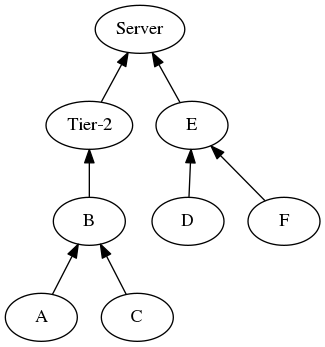
\includegraphics[width=0.35\linewidth]{./figures/methodology/spatial_correlation/dtstart2016-05-01_dtend2016-05-11_NRIDTCLDM031_graph_anonymized.png}
    \caption{User-groups structure.}
\label{fig:real_graph}
\end{figure}%

Since the links were oriented from the end-users to the server,
it is possible to model this structure as a DAG\@. The zero
indegree vertexes indicate equipments that only appear as the first hop,
however, an internal vertex can be a first hop in a traceroute.
Considering an arc (A, B), all users who belong to A also belong to B,
but the inverse is not necessarily true.

During the End-Users Filtering step, some clients are removed due to traceroute
inconsistencies~\cite{avoiding_traceroute_anomalies_with_paris_traceroute}.
As an example, there are cases in which the same equipment appears in different
hops of the same end-user traceroute. Also,
the measurement software limits the maximum number of hops, then,
scenarios in which the traceroute doesn't reach the server are discarded.
Since routing tables can be updated, after the Tier-2 vertexes compression,
it is only considered clients with static traceroutes
during the specified time period.
Situations characterized by Tier-2 routers that doesn't appear as consecutive
elements in the traceroute are also deleted.

\section{Events Times Correlation}
\label{sec:events_times_correlation}

The motivation of this mechanism is to infer network events that can explain
end-users events of an user-group.

There are two main reasons to detect the same network event, such as an
equipment failure, at different times in different clients. The first one is
related to the fact that the time series are not regularly sampled. The second
one is due to the change point detection algorithm behavior.
Therefore, a procedure to group end-users events based on their type and time,
should be flexible enough to take into consideration time delay effects. Also,
it must be robust to deal with multiple change points per time series.

In order to relax a change point location, a detected change point is
transformed into an interval according to a time tolerance.
Therefore, given a parameter $\delta$, a change point identified at
time $t$ implies in the existence of a change point within
$[t - \delta, t + \delta]$. To be consistent,
change point algorithms must report locations separated by more than
$2 \delta$ time units. In general, the algorithms presented in
Chapter~\ref{chap:change_point_detection}
can be adapted to respect this restriction. However, this can also be
achieved by the following post processing step:
sweeping time from left to right, if two
points are at most $2 \delta$ time units apart, then the right one is removed.

Consequently, the problem can be defined as selecting a set of network events,
that explain all end-users events. It is important to note that events are
defined only by their time and type.
An end-user event is explained by a network event if they have the same type,
and the end-user event time is inside the network event time interval.
This problem has several possible solutions, and the comparison between
them is subjective. As an example, not
necessarily selecting the minimum number of network events that cover all
end-user events is the most appropriate answer.

To this goal, it was developed a heuristic inspired in the Inexact Voting in
Totally
Ordered Space problem~\cite{voting_algorithms}. In this problem, people
vote in a single point in the real line. Also considering a $\delta$
parameter, the objective is to
select the interval with the greatest number of voters.

The created greedy procedure, called here as Multiple Inexact Voting in Totally
Ordered Space, is specified in
Algorithm~\ref{alg:multiple_inexact_voting_totally_ordered_space}

\begin{algorithm}[H]
\caption{Multiple Inexact Voting in Totally Ordered Space}
\label{alg:multiple_inexact_voting_totally_ordered_space}
    \begin{algorithmic}[1]
        \State{Let $l$ be the end-users events of a specific type sorted by
        time}
        \While{$l$ is not empty}
            \State{Considering only the events in $l$,
            select the interval $d$ with the greatest number of
            end-users events,
            in which all these events are at most $2 \delta$ apart.
            In case of ties, select the left most one}
            \State{Report the mean time of
            the $d$ extremes as the network event time}
            \State{Remove all end-users events from $l$ that are in $d$}
        \EndWhile{}
    \end{algorithmic}
\end{algorithm}

It is possible to note that, in each iteration the procedure solves an instance
of the Inexact Voting in Totally Ordered Space problem.
The proposed algorithm is executed three times in every user-group,
one for each event type.

A more straightforward solution, that was not used in this work, is to create
regular time-bins, and interpret all end-users events that occur at the same
bin as a common network event.
However, this strategy can introduce
discontinuities. If a network event occurs in the end/beginning of a time-bin,
then it is likely to different end-user events, associated with this
network event, be located in different bins.

If co-occurrent events with the same type affect the same end-users set,
it is not possible to distinguish them. Nonetheless, the chances of
detecting different events at the same time can reduce with the increase
of the time series sampling frequency.

\section{Spatial-Time Correlation}
\label{sec:spatial_time_correlation}

This step matches network events from different user-groups to define
a set of feasible events locations.

It is not possible to check if changes in round trip metrics, such as RTT,
are caused in the path from the end-user to the server or vice versa.
Therefore, correlate those metrics with the available traceroutes can lead to
erroneous or inconclusive outcomes. Also, the maximum achievable upstream
throughput can be affected by a service degradation on the path from the server
to the end-user, since losses of TCP's ACKs can influence the measurement
performance.
Hence, this work restricts to report possible events locations considering that
they are caused by equipments in the path from the end-user to the server.

The method expects that
a change point detection algorithm setup is able to detect all end-users
affected by a network event, or no end-user is identified.
Besides, with exception of the Tier-2 user-group, the mechanism supposes that
if an event occur in an user-group,
all traffic that goes through this cluster is affected by the event. Since
there is a direct connection between an user-group and an unique network
equipment, this is a reasonable hypothesis.

In the first reasoning part, it will be processed cases without the
presence of the Tier-2 user-group. Also, it will be removed
traceroutes paths that doesn't start in a zero indegree vertex.
Additionally, it will be disregarded co-occurrent events with the same type.
Later, these restrictions will be removed and treated separately.
Unless stated differently, in the rest of this section is considered an
unique network event in the period of study.

The procedure starts analyzing zero indegree vertexes.
Suppose that only a proper subset of the clients that belong to a zero
indegree node perceive the event. In this situation, it is possible to affirm
that this vertex is not the cause of the event, since not all clients detected
it. For the same reason, the cause is not located in posterior nodes
in the path to server.
Then, if this set size is bigger than one, these end-users must share
a network equipment, which is the cause, that doesn't respond to traceroute
pings, and is located before the first hop. As an example,
this equipment can be a fiber node.

However, if all clients of the zero indegree vertex detect the event, then
there are three options:
this vertex can be the cause, or these end-users can share an equipment before
the first hop that explains the event,
or the cause is located after the first hop. Due to the
lack of information about the topology above the IP layer, the first two cases
can't be
distinguished. Nonetheless, to check the latter scenario, the same type of
analysis is applied to the next vertex in the path to the server. If not all
clients of the second hop detected this event, then it is surely located
in the first hop or before. Otherwise, the procedure continues to the next hop.

When applied to different zero indegree vertexes,
this method results in possible events locations that are prefixes of
the paths to the server.
Also, these prefixes can be correlated.
If different paths detect the same network
event, then they must share at least one equipment. The
ones that are not common can be discarded from the possible cause list, since
there are end-users that don't belong to them and still perceive the event.

Figure~\ref{fig:network_events_locations_examples} presents several topologies
and different network events. The gray vertexes indicate a network event
that occurred in this location.

\begin{figure}[H]
    \centering
    \makebox[\textwidth][c]{%
        \begin{subfigure}[b]{0.2\textwidth}
            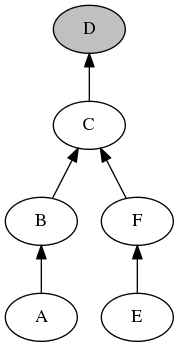
\includegraphics[width=\textwidth]{./figures/methodology/spatial_time_correlation/event_tree_graph_1.png}
            \caption{}\label{fig:network_events_locations_examples_1}
        \end{subfigure}
        \begin{subfigure}[b]{0.2\textwidth}
            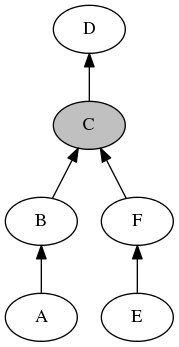
\includegraphics[width=\textwidth]{./figures/methodology/spatial_time_correlation/event_tree_graph_2.png}
            \caption{}\label{fig:network_events_locations_examples_2}
        \end{subfigure}%
        \begin{subfigure}[b]{0.3\textwidth}
            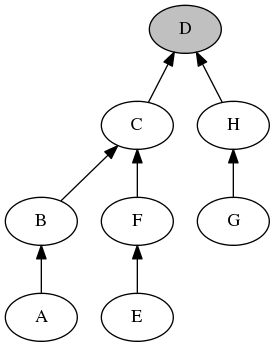
\includegraphics[width=\textwidth]{./figures/methodology/spatial_time_correlation/event_tree_graph_3.png}
            \caption{}\label{fig:network_events_locations_examples_3}
        \end{subfigure}
        \begin{subfigure}[b]{0.3\textwidth}
            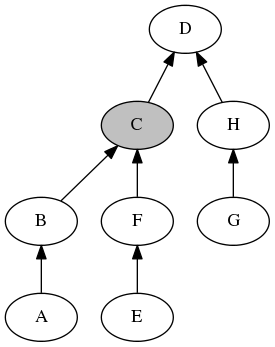
\includegraphics[width=\textwidth]{./figures/methodology/spatial_time_correlation/event_tree_graph_4.png}
            \caption{}\label{fig:network_events_locations_examples_4}
        \end{subfigure}%
    }
    \caption{Network event location examples.}
\label{fig:network_events_locations_examples}
\end{figure}%

In Figure~\ref{fig:network_events_locations_examples_1}, the analysis
starting at vertex A results in the following feasible event locations,
\{A, B, C, D\}. The reasoning through node E leads to
\{E, F, C, D\}. Correlating both results, the possible locations are \{C, D\}.
Figure~\ref{fig:network_events_locations_examples_2} presents a scenario with
the same conclusion.

In Figure~\ref{fig:network_events_locations_examples_3}, the analysis made
through the zero indegree vertexes result in the paths from them to the server.
Matching the outcomes, the D vertex is the only possible event location.

In Figure~\ref{fig:network_events_locations_examples_4}, the reasoning through
node G doesn't detect the event. The analysis in A finds \{A, B, C\}. Through
node E, \{E, F, C\} is the result.
Correlating the outcomes, C is the only feasible event location.

The previous analysis can't be fully applied in situations with the Tier-2
user-group.
As an example, suppose two geographically distant end-users in an OFF-NET case.
The packets from these two users can go through completely different routers in
the Tier-2 ISP\@. Then, it is possible that an event in the Tier-2 ISP only
affects one of the users, which contradicts one of the established suppositions.
To overcome this issue, when analyzing a path, if an event can be located in the
previous hop of the Tier-2 user-group, then the event can also be located at
the Tier-2 vertex, even considering that not all end-users of this user-group
perceive the event.

Now, suppose paths that doesn't start in zero indegree vertexes.
After the previous analysis,
if all clients of the first hop user-group detect the event, then this
path was already treated. Otherwise, the end-users that detected the event
share an equipment before the first hop,
that doesn't answer to traceroute pings, and is the cause.

If there are co-occurrent events with the same type, the complete procedure can
result in a wrong outcome. Figure~\ref{fig:network_events_locations_examples_5}
illustrates this case.

\begin{figure}[H]
    \centering
    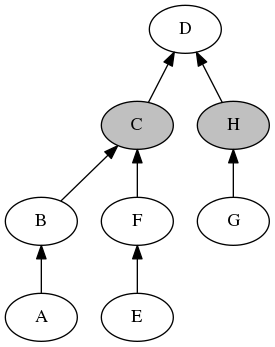
\includegraphics[width=0.35\linewidth]{./figures/methodology/spatial_time_correlation/event_tree_graph_5.png}
    \caption{Co-occurent events.}
\label{fig:network_events_locations_examples_5}
\end{figure}%

Through node A, the feasible locations are \{A, B, C, D\}.
Checking E, the result is \{E, F, C, D\}.
In vertex G, the outcome is \{G, H, D\}.
The paths results correlation leads to the location D, which is a mistake.
Therefore, when considering co-occurrent events with the same type, the step of
matching the conclusions of different paths must not be applied, and the
union of these results should be the final outcome.

From this procedure, it is possible to formulate a
problem to define the minimum number of end-users to be monitored, and their
placement to localize events with the minimum number of feasible locations.

\section{Change Point Detection Issues}

As stated in Chapter~\ref{chap:change_point_detection}, one of the main issues
of this work is the algorithms and parameters selection.
In general, this process requires a dataset to enable the evaluation of an
algorithm setup.

There are several approaches to construct a
change points dataset in the literature.
Some works create simulated time series, in which distinct segments are sampled
by the same generative model with different
parameters~\cite{change_point_detection_in_time_series_data_by_relative_density_ratio_estimation}.
In general, this type of data is more easily handled by change point detection
algorithms, since some methods assume the same models used in the dataset
building process. Also, real data can have complex characteristics that are
difficult to be reproduced by generative models. Another strategy is to join
segments from different real time series with different
characteristics~\cite{inertial_hidden_markov_models_modeling_change_in_multivariate_time_series}.
However, this can introduce unreal change points scenarios. Since one of
the goals of this work is to deal directly with real data,
this approach was discarded.

When the latent information of the time series are available, and if there is a
complete knowledge of what configurations changes in the latent state impact
data, it is possible to check the change points only analyzing this underlying
information. As an example, consider a time series that represents the cardiac
frequency of a soccer player during a match. Also, consider that in this
controlled environment, the only causes of changes in the cardiac frequency are
the variations of physical activities, such as starting or stopping to run.
Therefore,
it is possible to use the times in which a player changed his movement behavior
as the change points, without even analyzing the time series. However, in the
application domain of the present work, this approach would be impractical.
First, this would need the expertise of how the configurations of network
topology, routers congestion, physical equipment problems, among other features,
affect the different end-to-end QoS metrics.
Second, this kind of information is absent in the dataset, and would be too
complex to collect it.

Another way is to use visual annotations,
as it was done
in~\cite{learning_sparse_penalties_for_change_point_detection_using_max_margin_interval_regression}.
Also, manual labeling is usual for anomaly identification in Internet traffic
traces~\cite{webclass_adding_rigor_to_manual_labeling_of_traffic_anomalies}.
In this strategy, an application domain expert is exposed to a time series,
and visually indicates his opinion about the change points locations.

It is known that visual inspection methods can bring erroneous
conclusions~\cite{leveraging_cloud_data_to_mitigate_user_experience_from_breaking_bad},
and also amplify subjectivity, however, to better understand the problem, this
approach was experimented in this work.

Through a web system a user freely marked the change points with a mouse.
The fact that data is not regularly sampled in time could bring an unwanted
visual change perception. Therefore, the X axis of the displayed time series
represented only the temporal order of the measures.
It was only presented raw
loss fraction time series with 10 days of data.
Also, it was selected the ones that have at
least 85\% of the maximum possible number of points during the specified period,
considering that data is sampled at most two times in a hour. Change points can
be interpreted as rare events in this dataset, and several data streams have
almost
all measures with zero losses. Therefore, to increase the entropy,
it was selected time series that have at least one window of length 48 with
more than 5 measures with loss fraction larger than 0.01.

Additionally, it was provided a set of tips to the specialist:

\begin{itemize}
    \item In the case of packet loss fraction, mean changes between 0 and 0.1
    are more sensible to the end users.
    \item The time axis only represents the temporal order of the measurements.
    However, in general, consecutive points in time axis are separated by 30
    minutes.
    \item Outlier is not a statistical change. An outlier is an observation that
    lies outside the overall pattern of a distribution.
\end{itemize}

Figure~\ref{fig:survey_system} presents a system snapshot.
The vertical red line means that the user marked a change point in that
position.

\begin{figure}[H]
    \centering
    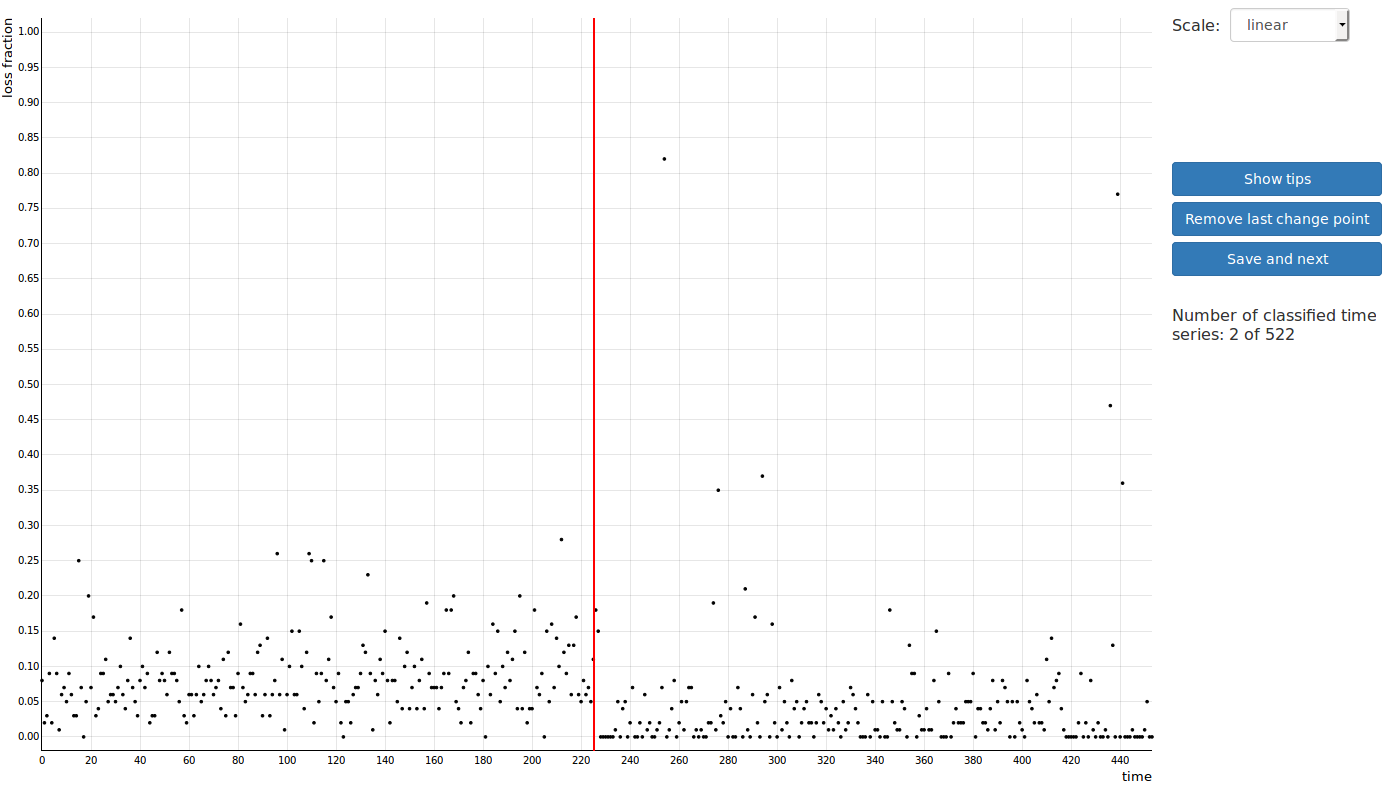
\includegraphics[width=0.9\linewidth]{./figures/methodology/supervised_learning_try/survey_system.png}
    \caption{Survey system snapshot.}
\label{fig:survey_system}
\end{figure}%

Six specialists with experience in network measurements and statistical
modeling, but without background in change point detection, classified 71 time
series.
To analyze the agreement between different users classifications,
for each time series, was applied the Events Times Correlation
procedure~\ref{sec:events_times_correlation}. Therefore, it was
considered that each specialist voted to a set of change points positions.
The time tolerance was set to 7 hours, which means at most 14 consecutive
points.

Then, for each change point voted at least once, it was counted the number of
specialists that voted in that location.
Figure~\ref{fig:classifications_per_vote} shows the histogram of this counting.

\begin{figure}[H]
    \centering
    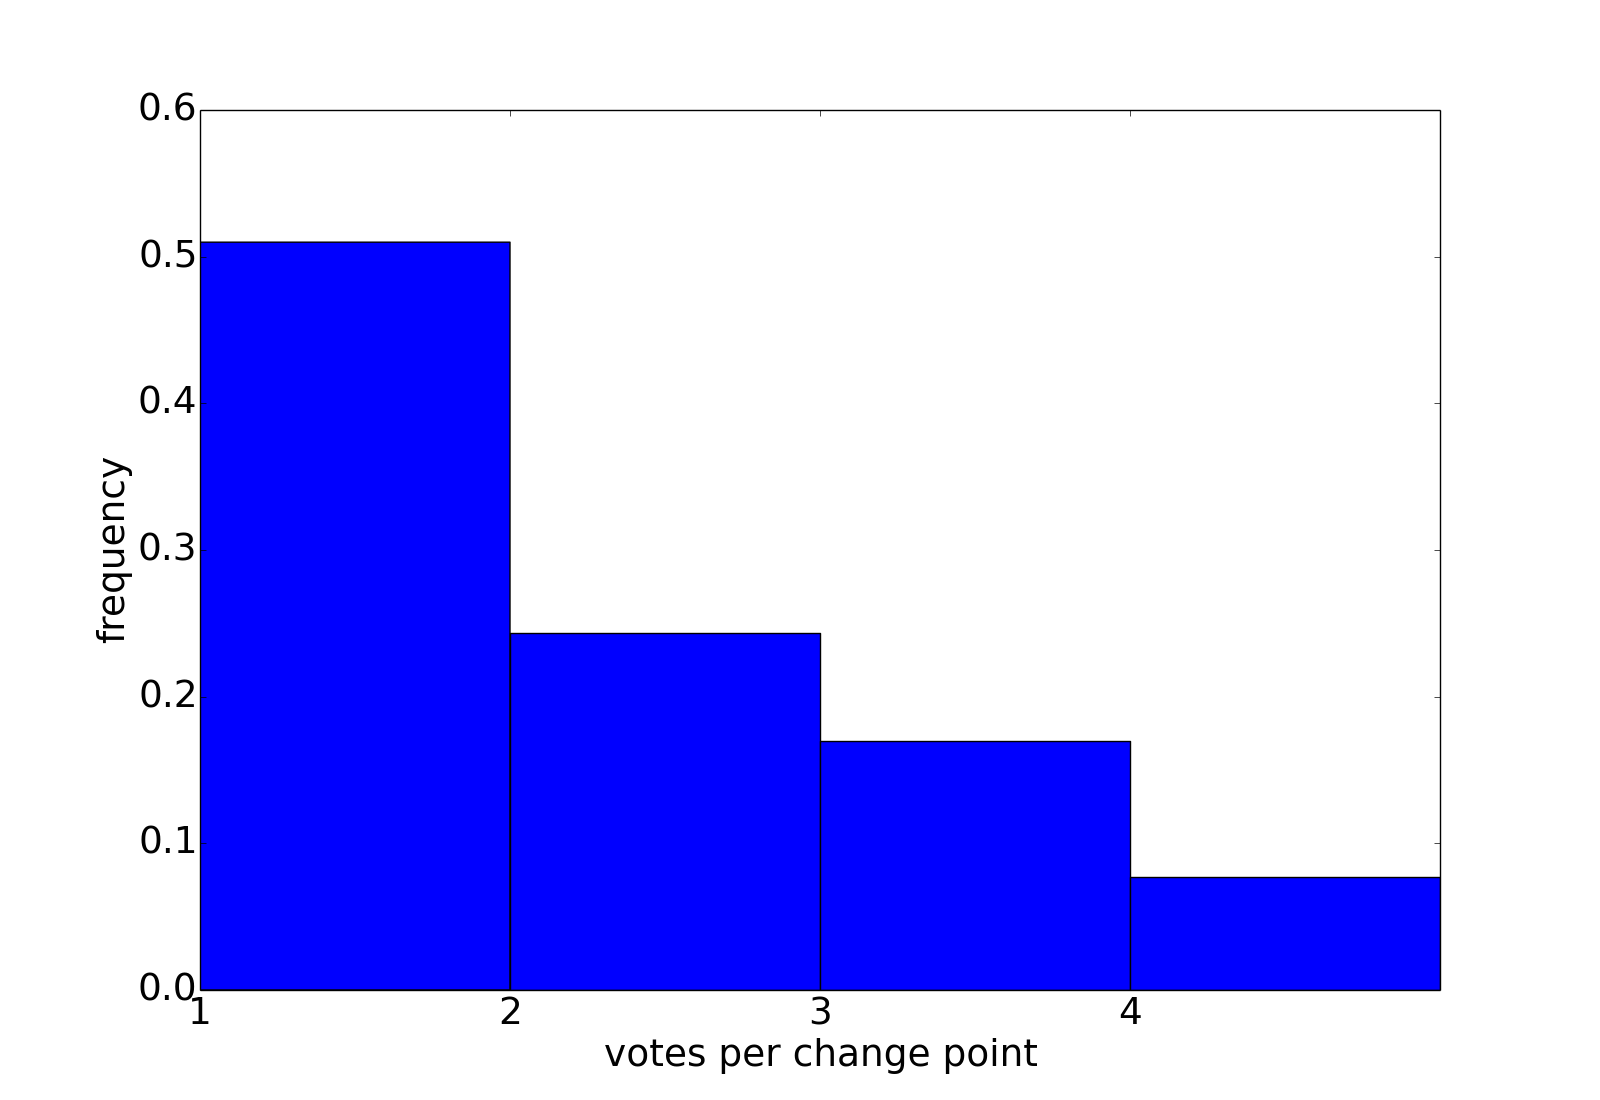
\includegraphics[width=0.7\linewidth]{./figures/methodology/supervised_learning_try/cnt_classifications_per_vote.png}
    \caption{Number of votes per change point histogram.}
\label{fig:classifications_per_vote}
\end{figure}%

It is possible to note that, 44\% of the change points were only voted by
a single user, and only 23\% were voted by the majority (more than 3 votes).
Therefore, in general, the consensus of change point locations is low.

In Figure~\ref{fig:classification_match} is presented the specialists
classifications in a time series with a high level of agreement on the change
points locations.

\begin{figure}[H]
    \centering
    \makebox[\textwidth][c]{%
        \begin{subfigure}[b]{0.55\textwidth}
            \includegraphics[width=\textwidth]{{./figures/methodology/supervised_learning_try/cnt6_serverNHODTCSRV04_mac64:66:B3:A6:BC:B8_dtstart2016-05-01_dtend2016-05-11/rosam@land.ufrj.br}.png}
            \caption{Specialist 1}\label{fig:classification_match_1}
        \end{subfigure}
        \begin{subfigure}[b]{0.55\textwidth}
            \includegraphics[width=\textwidth]{{./figures/methodology/supervised_learning_try/cnt6_serverNHODTCSRV04_mac64:66:B3:A6:BC:B8_dtstart2016-05-01_dtend2016-05-11/gustavo.santos@tgr.net.br}.png}
            \caption{Specialist 2}\label{fig:classification_match_2}
        \end{subfigure}
    }
    \makebox[\textwidth][c]{%
        \begin{subfigure}[b]{0.55\textwidth}
            \includegraphics[width=\textwidth]{{./figures/methodology/supervised_learning_try/cnt6_serverNHODTCSRV04_mac64:66:B3:A6:BC:B8_dtstart2016-05-01_dtend2016-05-11/guisenges@land.ufrj.br}.png}
            \caption{Specialist 3}\label{fig:classification_match_3}
        \end{subfigure}
        \begin{subfigure}[b]{0.55\textwidth}
            \includegraphics[width=\textwidth]{{./figures/methodology/supervised_learning_try/cnt6_serverNHODTCSRV04_mac64:66:B3:A6:BC:B8_dtstart2016-05-01_dtend2016-05-11/gabriel.mendonca@tgr.net.br}.png}
            \caption{Specialist 4}\label{fig:classification_match_4}
        \end{subfigure}
    }
    \makebox[\textwidth][c]{%
        \begin{subfigure}[b]{0.55\textwidth}
            \includegraphics[width=\textwidth]{{./figures/methodology/supervised_learning_try/cnt6_serverNHODTCSRV04_mac64:66:B3:A6:BC:B8_dtstart2016-05-01_dtend2016-05-11/edmundosilva@gmail.com}.png}
            \caption{Specialist 5}\label{fig:classification_match_5}
        \end{subfigure}
        \begin{subfigure}[b]{0.55\textwidth}
            \includegraphics[width=\textwidth]{{./figures/methodology/supervised_learning_try/cnt6_serverNHODTCSRV04_mac64:66:B3:A6:BC:B8_dtstart2016-05-01_dtend2016-05-11/edmundo@land.ufrj.br}.png}
            \caption{Specialist 6}\label{fig:classification_match_6}
        \end{subfigure}
    }
    \caption{Classifications agreements.}
\label{fig:classification_match}
\end{figure}%

Figure~\ref{fig:classification_mismatch} shows a time series with
several disagreements.
It was verified that this case is the most representative in the
constructed dataset, fact that corroborates with the problem subjectiveness.

\begin{figure}[H]
    \centering
    \makebox[\textwidth][c]{%
        \begin{subfigure}[b]{0.55\textwidth}
            \includegraphics[width=\textwidth]{{./figures/methodology/supervised_learning_try/cnt6_serverCTBDTCLDM91_mac64:66:B3:A6:B7:BC_dtstart2016-05-01_dtend2016-05-11/rosam@land.ufrj.br}.png}
            \caption{Specialist 1}\label{fig:classification_mismatch_1}
        \end{subfigure}
        \begin{subfigure}[b]{0.55\textwidth}
            \includegraphics[width=\textwidth]{{./figures/methodology/supervised_learning_try/cnt6_serverCTBDTCLDM91_mac64:66:B3:A6:B7:BC_dtstart2016-05-01_dtend2016-05-11/gustavo.santos@tgr.net.br}.png}
            \caption{Specialist 2}\label{fig:classification_mismatch_2}
        \end{subfigure}
    }
    \makebox[\textwidth][c]{%
        \begin{subfigure}[b]{0.55\textwidth}
            \includegraphics[width=\textwidth]{{./figures/methodology/supervised_learning_try/cnt6_serverCTBDTCLDM91_mac64:66:B3:A6:B7:BC_dtstart2016-05-01_dtend2016-05-11/guisenges@land.ufrj.br}.png}
            \caption{Specialist 3}\label{fig:classification_mismatch_3}
        \end{subfigure}
        \begin{subfigure}[b]{0.55\textwidth}
            \includegraphics[width=\textwidth]{{./figures/methodology/supervised_learning_try/cnt6_serverCTBDTCLDM91_mac64:66:B3:A6:B7:BC_dtstart2016-05-01_dtend2016-05-11/gabriel.mendonca@tgr.net.br}.png}
            \caption{Specialist 4}\label{fig:classification_mismatch_4}
        \end{subfigure}
    }
    \makebox[\textwidth][c]{%
        \begin{subfigure}[b]{0.55\textwidth}
            \includegraphics[width=\textwidth]{{./figures/methodology/supervised_learning_try/cnt6_serverCTBDTCLDM91_mac64:66:B3:A6:B7:BC_dtstart2016-05-01_dtend2016-05-11/edmundosilva@gmail.com}.png}
            \caption{Specialist 5}\label{fig:classification_mismatch_5}
        \end{subfigure}
        \begin{subfigure}[b]{0.55\textwidth}
            \includegraphics[width=\textwidth]{{./figures/methodology/supervised_learning_try/cnt6_serverCTBDTCLDM91_mac64:66:B3:A6:B7:BC_dtstart2016-05-01_dtend2016-05-11/edmundo@land.ufrj.br}.png}
            \caption{Specialist 6}\label{fig:classification_mismatch_6}
        \end{subfigure}
    }
    \caption{Classifications disagreements.}
\label{fig:classification_mismatch}
\end{figure}%

Also, it is possible to note that some users apparently changed their
classification pattern in the same time series. As an example,
Figure~\ref{fig:diff_class_same_time_series} presents two specialists that fits
this description. Also, in general, users changed their classification pattern
in different time series.

\begin{figure}[H]
    \centering
    \makebox[\textwidth][c]{%
        \begin{subfigure}[b]{0.55\textwidth}
            \includegraphics[width=\textwidth]{{./figures/methodology/supervised_learning_try/cnt6_serverNHODTCSRV04_mac64:66:B3:A6:B6:36_dtstart2016-05-01_dtend2016-05-11/rosam@land.ufrj.br}.png}
            \caption{Specialist 1}\label{fig:diff_class_same_time_series_1}
        \end{subfigure}
        \begin{subfigure}[b]{0.55\textwidth}
            \includegraphics[width=\textwidth]{{./figures/methodology/supervised_learning_try/cnt6_serverNHODTCSRV04_mac64:66:B3:A6:B6:36_dtstart2016-05-01_dtend2016-05-11/edmundo@land.ufrj.br}.png}
            \caption{Specialist 6}\label{fig:diff_class_same_time_series_6}
        \end{subfigure}
    }
    \caption{Different classification pattern in the same time series.}
\label{fig:diff_class_same_time_series}
\end{figure}%

Since this initial experiment resulted in a noisy dataset, in which change
points probably don't reflect real network events, this strategy was aborted.
Also, it would be difficult to scale the study to include more
specialists and time series.

It is important to note that the algorithms described in
Chapter~\ref{chap:change_point_detection} are unsupervised methods.
Once a change point dataset is constructed, it is possible to apply supervised
learning procedures, which are not much explored in the change
point detection literature.

\section{Differences to Previous Systems}

The proposed data analytics architecture has several similarities with the
projects described in Chapter~\ref{chap:literature_review}.

As with Argus and NetNorad, this work clusters end-users in user-groups, however
with finer topology granularity. Also, to increase the system's scalability,
NetNorad and Argus use this grouping to reduce the number of tracked time
series. This strategy was not applied in this project,
since the finer granularity requires more time series to be spread in different
network locations, and the current dataset has a low number of end-users.

To detect faults, Argus applies an anomaly detection procedure, but the present
work uses a change point detection method. The difference between
these two problems is subtle, and can be fuzzy in the literature. The
anomaly detection assumes that a standard pattern is already known or
is identified by the procedure, then the goal is to find when the data
stream
deviates from it's standard. The change point detection only seeks for
points where the statistical properties change, and doesn't take into
consideration a standard time series behavior.

Additionally, beyond the network edge point of view, Argus and NetNorad
uses some internal network information, which is absent in the present work.
